%% Creator: Inkscape inkscape 0.48.0, www.inkscape.org
%% PDF/EPS/PS + LaTeX output extension by Johan Engelen, 2010
%% Accompanies image file 'cyclotrone_lines.ps' (pdf, eps, ps)
%%
%% To include the image in your LaTeX document, write
%%   \input{<filename>.pdf_tex}
%%  instead of
%%   \includegraphics{<filename>.pdf}
%% To scale the image, write
%%   \def\svgwidth{<desired width>}
%%   \input{<filename>.pdf_tex}
%%  instead of
%%   \includegraphics[width=<desired width>]{<filename>.pdf}
%%
%% Images with a different path to the parent latex file can
%% be accessed with the `import' package (which may need to be
%% installed) using
%%   \usepackage{import}
%% in the preamble, and then including the image with
%%   \import{<path to file>}{<filename>.pdf_tex}
%% Alternatively, one can specify
%%   \graphicspath{{<path to file>/}}
%% 
%% For more information, please see info/svg-inkscape on CTAN:
%%   http://tug.ctan.org/tex-archive/info/svg-inkscape

\begingroup
  \makeatletter
  \providecommand\color[2][]{%
    \errmessage{(Inkscape) Color is used for the text in Inkscape, but the package 'color.sty' is not loaded}
    \renewcommand\color[2][]{}%
  }
  \providecommand\transparent[1]{%
    \errmessage{(Inkscape) Transparency is used (non-zero) for the text in Inkscape, but the package 'transparent.sty' is not loaded}
    \renewcommand\transparent[1]{}%
  }
  \providecommand\rotatebox[2]{#2}
  \ifx\svgwidth\undefined
    \setlength{\unitlength}{243.9203125pt}
  \else
    \setlength{\unitlength}{\svgwidth}
  \fi
  \global\let\svgwidth\undefined
  \makeatother
  \begin{picture}(1,0.73633127)%
    \put(0,0){\includegraphics[width=\unitlength]{pics/cyclotrone_lines.ps}}%
    \put(0.5,0.00334702){\color[rgb]{0,0,0}\makebox(0,0)[lb]{\smash{$f/f_{ce}$}}}%
    \put(0.14246156,0.08534101){\color[rgb]{0,0,0}\makebox(0,0)[lb]{\smash{$0$}}}%
    \put(0.2882347,0.08534101){\color[rgb]{0,0,0}\makebox(0,0)[lb]{\smash{$0.5$}}}%
    \put(0.46772147,0.08483015){\color[rgb]{0,0,0}\makebox(0,0)[lb]{\smash{$1$}}}%
    \put(0.61302379,0.08534101){\color[rgb]{0,0,0}\makebox(0,0)[lb]{\smash{$1.5$}}}%
    \put(0.94574304,0.08534101){\color[rgb]{0,0,0}\makebox(0,0)[lb]{\smash{$2.5$}}}%
    \put(0.7941048,0.08534101){\color[rgb]{0,0,0}\makebox(0,0)[lb]{\smash{$2$}}}%
    \put(0.02741034,0.3765521){\color[rgb]{0,0,0}\rotatebox{90}{\makebox(0,0)[lb]{\smash{$\Delta{}B$\,(мГс)}}}}%
    \put(0.04,0.17834724){\color[rgb]{0,0,0}\makebox(0,0)[lb]{\smash{$-12$}}}%
    \put(0.04,0.26264651){\color[rgb]{0,0,0}\makebox(0,0)[lb]{\smash{$-10$}}}%
    \put(0.063,0.34669035){\color[rgb]{0,0,0}\makebox(0,0)[lb]{\smash{$-8$}}}%
    \put(0.067,0.51476042){\color[rgb]{0,0,0}\makebox(0,0)[lb]{\smash{$-4$}}}%
    \put(0.069,0.59856645){\color[rgb]{0,0,0}\makebox(0,0)[lb]{\smash{$-2$}}}%
    \put(0.11,0.68320603){\color[rgb]{0,0,0}\makebox(0,0)[lb]{\smash{$0$}}}%
    \put(0.063,0.43298192){\color[rgb]{0,0,0}\makebox(0,0)[lb]{\smash{$-6$}}}%
    \put(0.88,0.29590222){\color[rgb]{0,0,0}\makebox(0,0)[lb]{\smash{$(1)$}}}%
    \put(0.88,0.24363105){\color[rgb]{0,0,0}\makebox(0,0)[lb]{\smash{$(2)$}}}%
    \put(0.88,0.19101547){\color[rgb]{0,0,0}\makebox(0,0)[lb]{\smash{$(3)$}}}%
  \end{picture}%
\endgroup
